\newpage
\section{Generator}
The purpose of this block is to convert rotational energy into electrical energy. Once converted, the electrical energy can be deposited in the Load System.

As the Generator was chosen by the customer and as it is pre-mounted on the Roll Stand, the block will not be designed but will be analysed instead.

\subsection{Implementation}
The Generator consists of a DC-motor which is mounted on the Roll Stand. The motor's rotor connected with a drive shaft through a gearing. This drive shaft runs through the Torque Sensor and connects with the Roll - which in turn can be rotated by a car (AU2).

\begin{figure}[H]
	\centering
	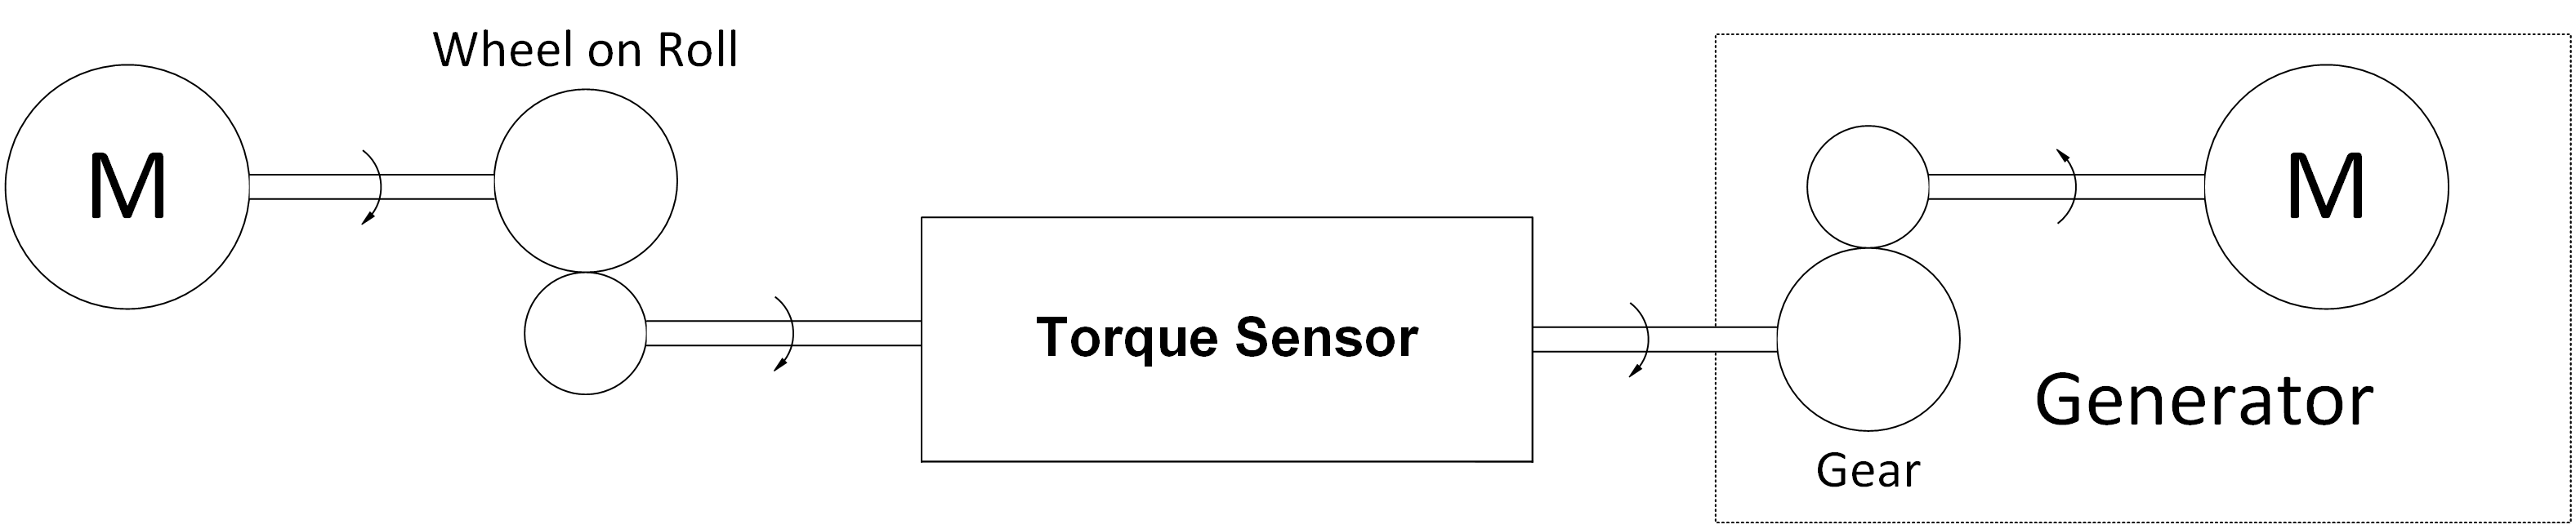
\includegraphics[width=1\linewidth]{Hardware/Pictures/Mechanical_Connections}
	\caption{Mechanical configuration in the Roll Stand}
	\label{fig:Generator_Implementation}
\end{figure}

\subsection{Analysis}
The Generator is built with a MAXON 200 Watt DC-motor with permanent magnets. When the motor's rotor is spun, a voltage drop will be created between the motor's positive and negative terminals. The voltage-drop depends on the the motor velocity constant k\textsubscript{e} which for the specified motor is given as:
\begin{equation}
	K_e = 248 \frac{rpm}{V}
\end{equation}

The maximum possible voltage-drop between the Generator's terminals, when AU2 is tested with Rolling Road, can be calculated by using the cruise speed (maximum velocity) of AU2. It is given as:
\begin{equation}
	v_{AU2} = 30 \frac{km}{t} = 8.33 \frac{m}{s}
\end{equation}

Due to the difference in diameter between AU2's wheel and the Roll creates a gearing ratio R\textsubscript{A} between the wheel's and the generator's angular velocity. This ratio can be determined by the diameters of the wheel and the Roll:
\begin{equation}
	\begin{split}
		d_{wheel} &= 478 mm\\
		d_{Roll} &= 152 mm
	\end{split}
\end{equation}

\begin{equation}
	\begin{split}
		R_A &= \frac{d_{wheel}}{d_{Roll}}\\
		R_A &= \frac{478 mm}{152 mm} = 3.15
	\end{split}
\end{equation}

As seen on \vref{fig:Generator_Implementation}, another gear is installed between the Torque Sensor's output and the Generator's input. This ratio is given as:
\begin{equation}
	R_B = 1:4.3
\end{equation}

The rotor's angular velocity, when AU2 runs at cruise speed, can be calculated using the gearing ratios. Angular velocity of the car's wheel:
\begin{equation}
	\begin{split}
		\omega_{wheel} &= \frac{v_{wheel}}{r_{wheel}} = \frac{v_{wheel}}{d_{wheel} \cdot 0.5}\\
		\omega_{wheel} &=
	\end{split}
\end{equation}

Angular velocity of the Roll:
\begin{equation}
	\begin{split}
		\omega_{Roll} &= \omega_{wheel} \cdot R_A\\
		\omega_{Roll} &=
	\end{split}
\end{equation}

Angular velocity of the Generator's rotor:
\begin{equation}
	\begin{split}
		\omega_{rotor} &= \omega_{Roll} \cdot R_B\\
		\omega_{rotor} &=
	\end{split}
\end{equation}

The induced voltage-drop between the terminals:
\begin{equation}
	\begin{split}
		V_b &= \frac{\omega_{rotor}}{k_e}\\
		V_b &=
	\end{split}
\end{equation}

\subsection{Unity test}
Text